\documentclass[aps,prl,5p,showpacs,showkeys,twocolumn]{revtex4-1}
\usepackage{hyperref}
\usepackage{graphicx}


\begin{document}
\title{Non-parabolicity and band gap renormalization in Si doped ZnO}
\author{R. E. Treharne}
\email[Corresponding Author: ]{R.Treharne@liverpool.ac.uk}
\affiliation{Stephenson Institute for Renewable Energy, University of Liverpool, UK}
\author{L. J. Phillips, K. Durose}
\affiliation{Stephenson Institute for Renewable Energy, University of Liverpool, UK}
\date{\today}
\begin{abstract}
\end{abstract}
\pacs{78.20.Jq, 88.66.sq, 81.15.-z}
\keywords{zinc oxide; magnetron sputtering; thin-film; doping; non-parabolicity, band gap normalisation}
\maketitle

\section{Introduction}



\section{Experimental Methods}

Films were deposited via RF magnetron sputtering using an AJA Phase II-J Orion system. The system was configured with a 'sputter-up' geometry with the substrate being suspended above two separate ceramic targets of ZnO and SiO$_2$ that were arranged off-centre and tilted at $5^{\circ}$ towards the middle of the substrate.  Soda-lime glass substrates (OptiWhite$^{TM}$, NSG) of size $100\times100\times4$ mm$^{3}$ were used throughout. They were cleaned by scrubbing with a nylon brush and a series of de-ionized water and isopropanol alcohol rinses followed by blow drying with a nitrogen gas jet. During deposition the ZnO and SiO$_2$ targets were sputtered from simultaneously using powers of $150$ W and $50$ W respectively. A growth pressure of 2mTorr Ar was used during deposition. The substrate temperature was maintained at $350\pm5^{\circ}$C during growth and the substrate was kept static (i.e was not rotated). Deliberate gradients of both thickness and composition were subsequently achieved across the resultant film to generate a `combinatorial' sample. A second film of pure SiO$_{2}$ was deposited under identical conditions (but without ZnO) to generate a reference film for calculating the \% wt. profile of SiO$_{2}$ in the co-sputtered film.

A Shimadzu UV-Vis-IR 3700 spectrophotometer with mapping capability was used to measure the transmittance of the co-sputtered film over the range 250 - 2500 nm. 289 spectra were taken in total at 5 mm increments over the full sample surface. At each of these 289 points the sheet resistance was also measured using a CMT-SR2000 4-point probe mapping system. Following transmittance and sheet resistance measurements the sample was cut into one hundred $10\times10$ mm$^2$ pieces. A selection of these pieces, 10 in total, were further scribed into four $5\times5$ mm$^2$ sections and Hall measurement were performed on each of these sections. The Hall measurement was performed with custom built equipment, provided by Semimetrics Ltd., using a field strength of 0.8 T.  Ellipsometry was performed on the same sections using a Woollam M2000-UI system. Ellipsometry was also used to map the thickness profile of the pure SiO$_{2}$ reference film.

\section{Results}\label{sec:2}

\subsection{Fitting of optical spectra}\label{sec:2.1}

Figure \ref{fig:1} shows a typical transmittance spectra taken from a single point on the combinatorial ZnO:Si sample. The full details of the model of the dielectric permittivity, $\varepsilon(\omega)$, used to fit the data are given in \cite{Treharne2012}. The key components of the model include: 1) a Lorentzian oscillator to account for the behaviour of the system's bound electrons and to provide a smoothly varying dielectric background over the range of interest ($250-2500$ nm), 2) an extended Drude model \cite{Mergel2002}, to characterise the system's free electron response, and 3) an inter-band transition model to account for the steep increase in the material's absorption coefficient ($\alpha \propto (E-E_G)^{1/2}$) in the vicinity of its direct band gap ($3.3 - 3.4$ eV). The two key parameters extractable from the dielectric model are the film's thickness, $d$, and plasma frequency, $\omega_{p}$, which is related directly to the carrier concentration according to
\begin{equation}
\omega_p = \sqrt{\frac{n_e e^2}{m_e \varepsilon_0}}
\end{equation}\label{eqn:1}
where $m_e$ is the effective electrons (expressed in units of the free electron mass, $m_0$) and $\varepsilon_0$ is the permittivity of free space.

Fitting was achieved by using a Nelder-Mead downhill simplex algorithm \cite{Nelder1965}, implemented via python script, to minimize the quantity
\begin{equation}
\chi^{2} = \sum_{i}^N\sqrt{\frac{y_i - O_i}{N^2}}
\end{equation}\label{eqn:2}
where $N$ is the total number of data points in the spectra, $O_i$ the observed transmittance at each wavelength over the range of interest, and $y_i$ the theoretical transmittance calculated using the transfer matrix method \cite{Macleod1986} for a single thin-film on a finite, transparent substrate.  The fitting algorithm was iterated until the relative fractional change in consecutive $\chi^2$ values was less than $1\times10^{-6}$. The fitting of all 289 transmittance spectra taken over the combinatorial sample was fully automated, the only user input required being initial estimate for film thickness at the point of the first spectrum. This automation ensured that the fitting of consecutive spectra was highly consistent. For all spectra, $\chi^2$ values of $<1$ were achieved indicating that all fits were as successful as that shown in figure \ref{fig:1}.





\section{Conclusions}

\begin{acknowledgements}

\end{acknowledgements}

\bibliography{ref}


\begin{figure}[0]
\centering
\caption{\label{fig:1}}
\end{figure}

\begin{figure}[p]
\centering
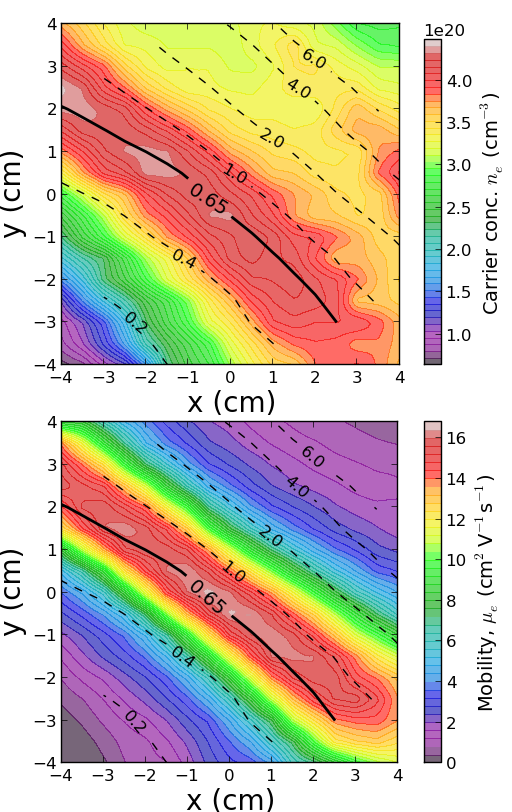
\includegraphics[width = \columnwidth]{figure2.png}
\caption{\label{fig:4} Contour maps of carrier concentration and mobility over the combinatorial sample. The (--) contour lines show an overlay of the \% wt. SiO$_{2}$ composition.}
\end{figure}

\begin{figure}[p]
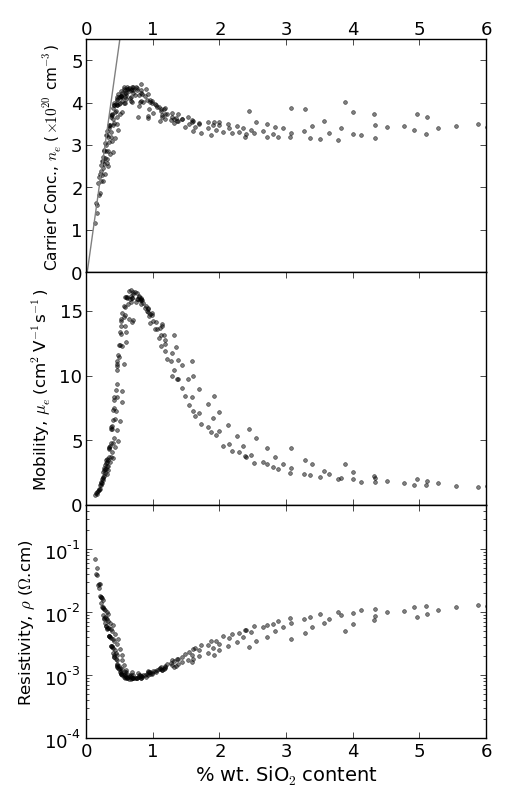
\includegraphics[width = \columnwidth]{figure3.png}
\caption{\label{fig:5} Distributions of carrier concentration, mobility and resistivity with respect to \% wt. SiO$_{2}$ content. The maximum values for $n_e$ ($4.4\times10^{20}$ cm$^{-3}$) and $\mu_{e}$ ($16.5$ cm$^{2}$V$^{-1}$s$^{-1}$) coincide with a composition of $0.65$\% wt. SiO$_{2}$. The solid straight line in the top plot shows the maximum theoretical carrier concentration with respect to SiO$_{2}$ content should every incorporated Si atom be substituted at a Zinc site and donate 2 carriers.}
\end{figure}

\begin{figure}[p]
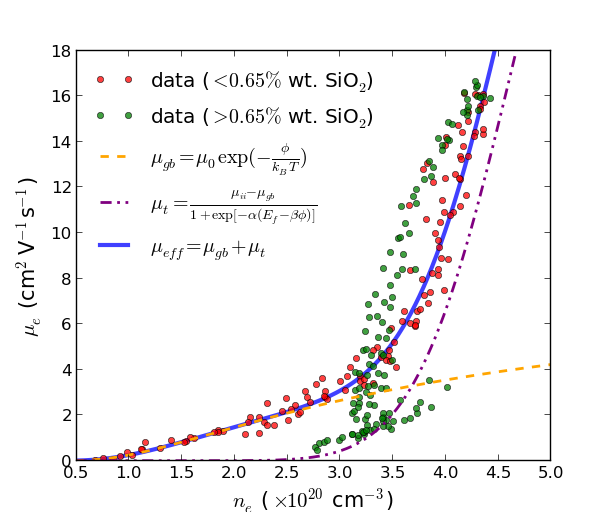
\includegraphics[width=1\columnwidth]{figure4.png}
\caption{\label{fig:6} }
\end{figure}

\begin{figure}[p]
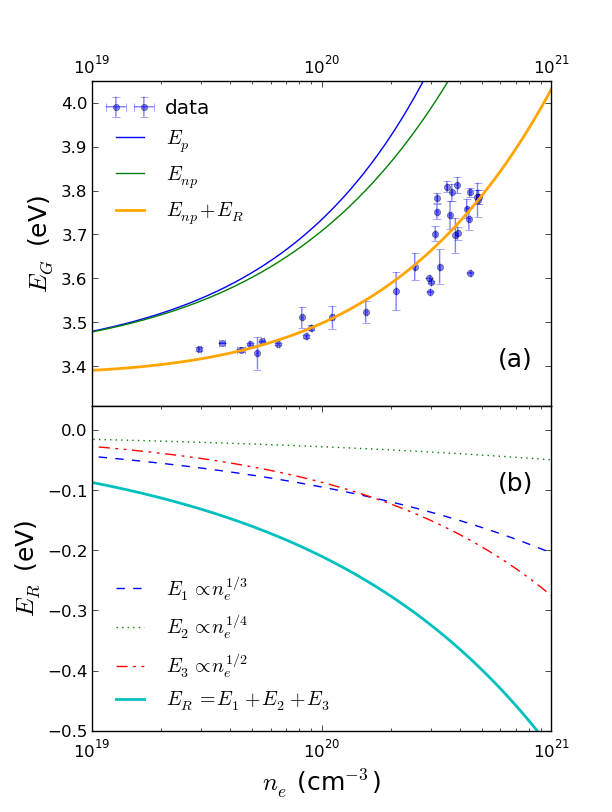
\includegraphics[width = \columnwidth]{figure5.png}
\caption{\label{fig:7}}
\end{figure}



\end{document}